\documentclass[aspectratio=1610,12pt,xcolor=dvipsnames]{beamer}
\mode<presentation>

% Respect chosen fonts (serif) and metrics
\usefonttheme{professionalfonts}
\renewcommand{\familydefault}{\rmdefault}

% Figures
\usepackage{graphicx}
\usepackage{float}

%% table
\usepackage{xcolor}
\usepackage{fancyhdr}
\usepackage{booktabs}
\usepackage[table]{xcolor}

% subsection page template
\setbeamertemplate{subsection page}
{
  \begin{centering}
    \vfill
    {\usebeamerfont{section title}\usebeamercolor[fg]{section title}\Large\insertsubsectionhead\par}
    \vfill
  \end{centering}
}
% section page template
\setbeamertemplate{section page}
{
  \begin{centering}
    \vfill
    {\usebeamerfont{section title}\usebeamercolor[fg]{section title}\Large\insertsectionhead\par}
    \vfill
  \end{centering}
}

%% footnote
\setbeamertemplate{footnote}{%
  \parindent 0em\noindent%
  \raggedright\insertfootnotemark\insertfootnotetext\par%
}

%% theme
\usetheme{default}
\useoutertheme{miniframes}
\definecolor{nagivation}{rgb}{0,0,0.35} % (typo kept if intentional)
\definecolor{main}{rgb}{0,0,0.5}
\setbeamercolor{structure}{bg=white,fg=nagivation}
\setbeamercolor{frametitle}{fg=nagivation}
\setbeamercolor{section in head/foot}{fg=white,bg=nagivation}
\setbeamertemplate{footline}[page number]
\setbeamertemplate{items}[circle]
\setbeamerfont{footnote}{size=\footnotesize}
\setbeamerfont{caption}{size=\footnotesize}
\setbeamertemplate{subsection in head/foot}{}%
\setbeamertemplate{subsection in head/foot shaded}{}%

%% font
\usepackage{dsfont}
\usepackage{newpxtext}
\usepackage{newpxmath}
\usepackage{amsmath}
\usepackage{caption}

% Math & bib
\usepackage{amsmath,amsfonts,amssymb,bm}
\DeclareMathOperator*{\argmin}{arg\,min}
\newcommand{\indep}{\perp\!\!\!\, \perp}
\usepackage{natbib}
\bibliographystyle{asr}
\setcitestyle{aysep={}}
\usepackage[english]{babel}

\makeatletter
\DeclareRobustCommand\citep
{\begingroup\scriptsize\color{gray}\NAT@swatrue\let\NAT@ctype\z@\NAT@partrue
    \@ifstar{\NAT@fulltrue\NAT@citetp}{\NAT@fullfalse\NAT@citetp}}
\makeatother

% Roman numerals macro
\newcommand{\rom}[1]{\uppercase\expandafter{\romannumeral #1\relax}}

%% Title
\title[CML]{SOC 690S: Machine Learning in Causal Inference\\[1.5pt]}
\subtitle{\large Week 2: Machine Learning Basics\\[-10pt]}

%% author
\author[Jiang] 
{\large Wenhao Jiang\vspace{-2em}}

%% affiliation
\institute[Duke]{}
\titlegraphic{
\includegraphics[height=1.4cm]{Misc/duke_logo.png}}

\date[Duke]
{\large Department of Sociology, Fall 2025}

\begin{document}

%%%%%%%%%%%%%%%%%%%%%%%%%%%%%%%%%%%%
%%%%%%%%Begin Main Content%%%%%%%%%%
%%%%%%%%%%%%%%%%%%%%%%%%%%%%%%%%%%%%

%% Title page %%
\begin{frame}
    \titlepage 
\end{frame}

\section{Motivation and High-Dimensional Data}

\begin{frame}
  \sectionpage
\end{frame}

\begin{frame}{Sample Sandwich Estimator Fails in High Dimension}

\begin{itemize}
    \item Last week, we discussed the problem of \textit{sample} linear regression in the high-dimensional regime ($p/n \not\to 0$)
    \item Even if the true \textit{data-generating process} (DGP) in the \textit{population} is correctly specified ($E[\hat \beta] = \beta$), high dimensionality causes problems for the sample regression 
    \item In particular, the variance of the OLS (sandwich) estimator is \textit{underestimated} and inconsistent at rate $\sqrt{p/n}$, because the \textit{sample} covariance matrix no longer converges to its \textit{population} counterpart—the \textit{Law of Large Numbers} fails under high-dimensional regime
    \begin{align*}
    \Big\|\tfrac{1}{n}\sum_{i=1}^n X_iX_i' - E[X_iX_i']\Big\|_{\mathrm{op}}
    &\sim \mathcal{O}_p\!\Big(\sqrt{\tfrac{p}{n}}\Big)
    \end{align*}
\end{itemize}
\end{frame}

\begin{frame}{Sample Sandwich Estimator is Inconsistent}

\begin{itemize}
    \item Indeed, in high-dimensional regimes, $\hat \beta$ is no longer $\sqrt{n}$-consistent
    \[
    \sqrt{n}(\hat{\beta}-\beta)\not\xrightarrow{d}
    \mathcal{N}\!\left(0,\;E[X_iX_i']^{-1}\,E[e_i^2 X_i X_i']\,E[X_iX_i']^{-1}\right)
    \]
    \item The estimation uncertainty does not vanish to 0 even if $n \rightarrow \infty$ when $p/n \not \to 0$
    \begin{itemize}
        \item The number of parameters grows with $n$
        \item The overall estimation uncertainty does not vanish
        \item $\hat\beta$ is unbiased but not consistent
    \end{itemize}
\end{itemize}

\end{frame}


\begin{frame}{Out-of-Sample Prediction is Poor in High Dimension}

\begin{itemize}
    \item Another perspective: the \textit{out-of-sample} prediction error relative to the true regression does not converge to 0 when $n \to \infty$ in high dimension \pause
    \item Suppose $\hat{\beta}$ is the OLS estimate, $E_X[\cdot]$ denotes averaging over fresh test samples from the population. The \textit{root mean square prediction error} (RMSE) satisfies the high-probability bound
    \[
    \sqrt{E_X\!\big[(X_i'\beta - X_i'\hat\beta)^2\big]}
    \lesssim\text{const}_{\alpha}\,\sqrt{E[e_i^2]}\,\sqrt{\tfrac{p}{n}}\,
    \]
    \item the inequality holds with probability approaching $1-\alpha$ as $n \rightarrow \infty$, where $\text{const}_{\alpha}$ is a constant that depends on the distribution $(Y,X)$ and $\alpha$ (see details on page 19 in \textcolor{nagivation}{CML} \textit{Theorem 1.2.1}) \pause
    \item In the low-dimensional case ($p/n \to 0$), RMSE $\to 0$
    \item In the high-dimensional case ($p/n \not\to 0$), the RMSE plateaus at a positive constant even as $n\rightarrow\infty$
\end{itemize}
\end{frame}


\begin{frame}{Motivation of Dimension Reduction}
\begin{itemize}
    \item This week, we introduce basic \textit{Machine Learning} (ML) methods to improve the prediction of $X_i'\hat{\beta}$ relative to $X_i'\beta$ (and thus $Y_i$) in high-dimensional data
    \begin{itemize}
        \item Why do we care about \textit{prediction} for new unseen data
        \item It measures the extent to which the conclusion drawn from the sample is \textit{generalizable}
    \end{itemize} \pause
    \item The most straightforward strategy is to reduce dimension, \textit{i.e.}, the number of covariates ($p$) in linear regression, without losing important ``information''
    \item This is \textit{not} about causal inference in the framework of \textit{potential outcome} yet, but using \textit{sample} linear regression to approximate the DGP and the parameters (under strong \textit{ignorability} assumption)
\end{itemize}
\end{frame}

\begin{frame}{Practical Reason of High Dimension I}

\begin{itemize}
    \item This curse of high dimension is not rare even if \textbf{I.} the DGP is correctly specified in the \textit{sample}
    \begin{itemize}
        \item In cross-country analysis of economic growth, there are many country-level characteristics that may significantly predict growth ($p>n$)
        \item In hard-to-reach population, researchers may want to collect as much individual-level information as possible ($n$ is limited, while $p$ may be large)
    \end{itemize}
\end{itemize}
    
\end{frame}

\begin{frame}{Practical Reason of High Dimension II}

\begin{itemize}
    \item High dimensionality may also arise when \textbf{II.} the data have large dimensional features—many covariates are available for use as regressors
    \begin{itemize}
        \item These features may not appear in DGP, but they may approximate many unobserved characteristics in DGP that we want to model
        \item In modeling the relationship between demand and price of a rare product ($n$ is not large in reality), we want to use as many information as possible, including using textual or image features in product description, even if some of them are just noises
        \item Including many regressors without selection risk high \textit{colinearity}
    \end{itemize}
\end{itemize}
\end{frame}

\begin{frame}{Practical Reason of High Dimension III}

\begin{itemize}
    \item High dimensionality may also arise when \textbf{III.} we want to allow more flexible and interactive relationship between regressors
    \begin{itemize}
        \item In modeling the relationship between gender and wage, we want to allow years of experience to have ``non-linear'' effects, years of education to be interacted with geographic indicators, etc.
        \item These ``non-linear'' features are called \textit{constructed} features or \textit{transformations}
        \begin{align*}
            X = T(W) = (T_1(W), T_2(W), ...,T_p(W))'
        \end{align*}
        \item \textit{Transformations} risk \textit{overfitting} the sample
    \end{itemize}
\end{itemize}
\end{frame}

\section{Penalized Regression}

\subsection{Least Absolute Shrinkage and Selection Operator (LASSO) as a Feature Selection Method}

\begin{frame}
  \subsectionpage
\end{frame}

\begin{frame}{LASSO Regression Basic Setup}

\begin{itemize}
    \item We consider a linear regression model
    \begin{align*}
        Y_i = X_i'\beta +e_i = \sum_{j=1}^{p}\beta_jX_{ij} + e_i, \quad e_i \perp X_i
    \end{align*}
    where $p$ is possibly much larger than $n$
    \item Classic OLS fails in these high-dimensional settings
    \begin{itemize}
        \item \textit{Out-of-sample} prediction error can be very high
        \item Model identification fails when the covariate matrix $rank>n$, or perfectly fits the sample data when $rank=n$
    \end{itemize}
\end{itemize}
\end{frame}

\begin{frame}{LASSO Regression Basic Setup}
    \begin{itemize}
        \item For simplicity, we assume regressors are centered and normalized (\textit{standardized}), such that $\beta_j$ are on the same scale (standard packages typically do this by default)
    \begin{align*}
        E[X_{ij}^2] = 1, \quad \text{as } V(X_{ij}^2)=1, E[X_{ij}]=0
    \end{align*}
        \item We assume \textit{population}-level DGP follows \textit{approximate sparsity}\footnote{Formally, the sorted absolute values of the coefficients decay quickly. The $j^{th}$ largest coefficient (in absolute value) denoted by $|\beta|_j$ obeys $|\beta|_j \leq Aj^{-a}, a >1/2$ for each $j$}
        \begin{itemize}
            \item There is a small group of regressors with relatively large coefficients whose use alone suffices to approximate the BLP $X_i'\beta$
            \item The rest of the regressors are assumed to have relatively small coefficients and contribute little to the approximation of the BLP
        \end{itemize}
    \end{itemize}
\end{frame}

\begin{frame}{LASSO Regression Basic Setup: Approximate Sparsity}
\begin{itemize}
    \item A classic example of \textit{approximate sparsity} is captured by regression coefficients of the form
    \begin{align*}
        \beta_j \propto 1/j^2, \quad j = 1,...,p
    \end{align*}
\end{itemize}
    \begin{figure}
        \centering
        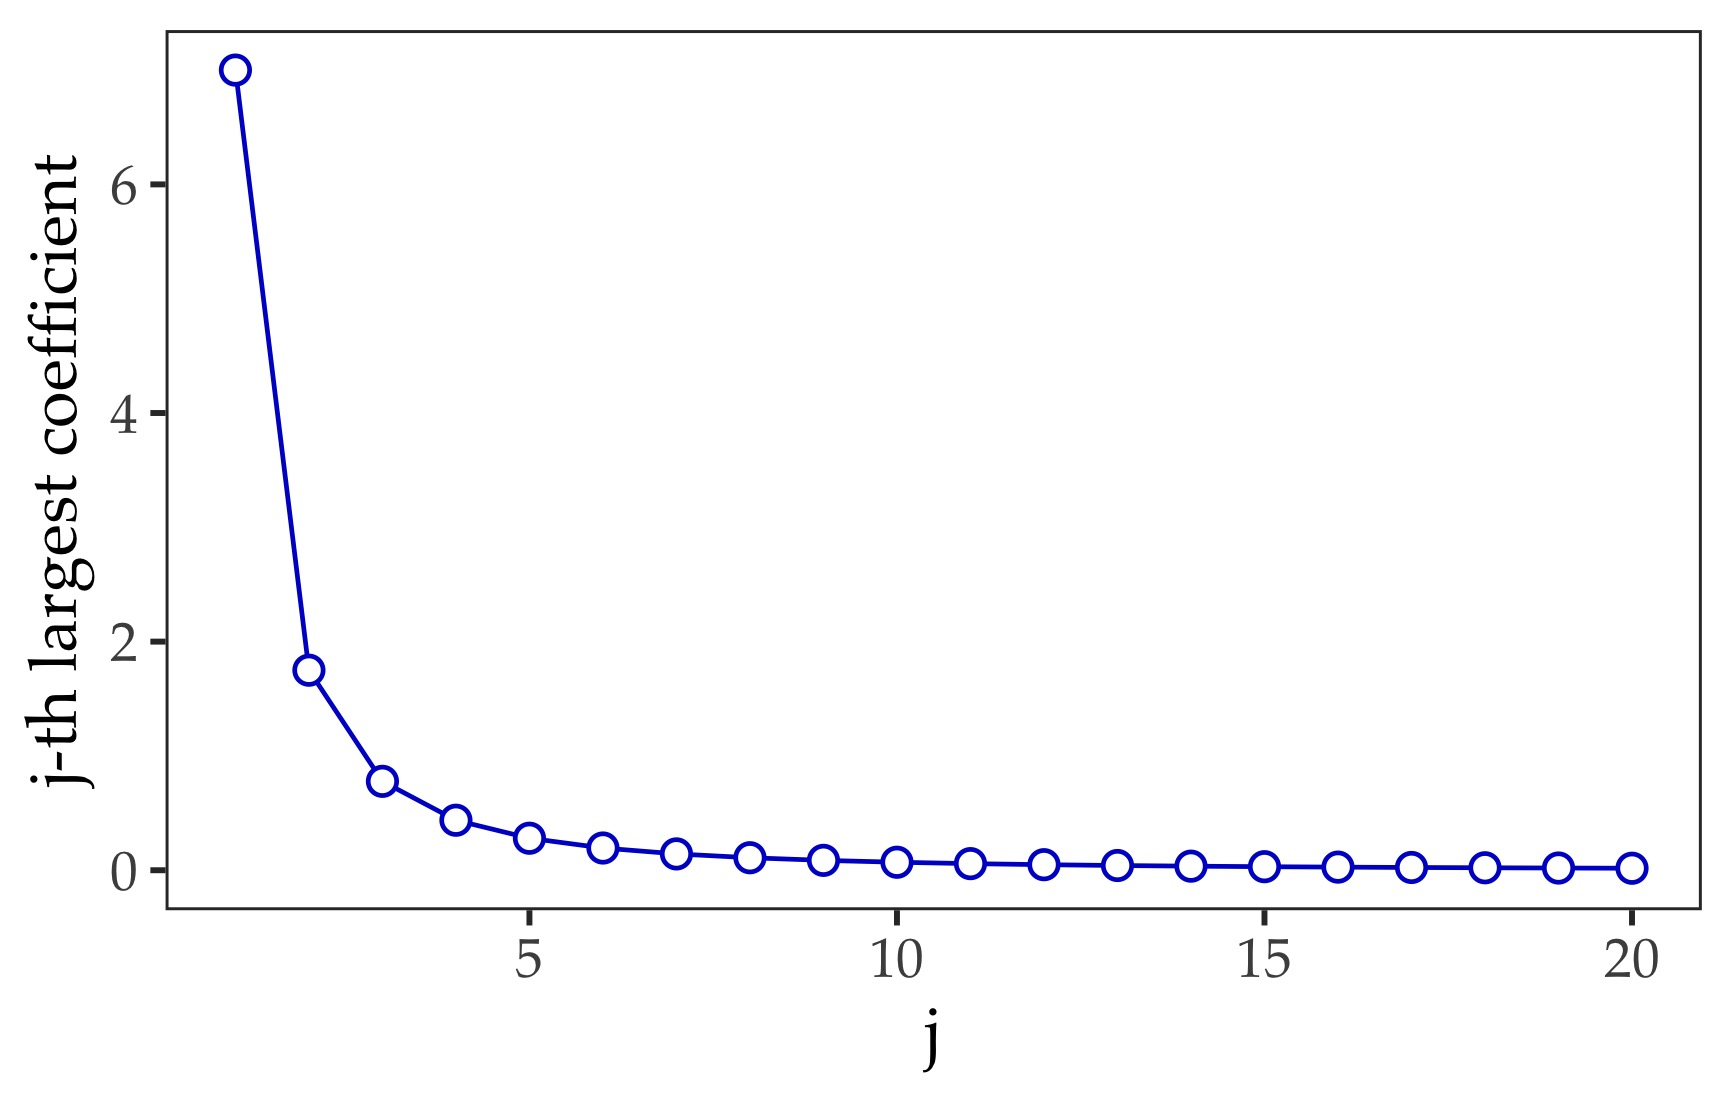
\includegraphics[width=0.6\linewidth]{Machine Learning Basics/Figures/Figure 3.1.jpg}
        \caption{Example of regression coefficients, $\beta_j \propto 1/j^2$ that satisfy approximate sparsity}
        \label{fig:figure3.1}
    \end{figure}
\end{frame}

\begin{frame}{LASSO Regression}
\begin{itemize}
    \item LASSO constructs $\hat \beta$ as the solution of the following \textit{penalized} least squares problem
    \begin{align*}
        \hat \beta = \argmin_{b\in\mathbb{R}^{p}}\sum_i^n(Y_i - X_i'b)^2 + \lambda \cdot \sum_{j=1}^{p}|b_j| \hat \psi_j
    \end{align*}
    \item The first term is the \textit{prediction} error
    \item The the second term is called a \textit{penalty term}, with \textit{penalty level} $\lambda$ and \textit{penalty loading} $\hat \psi_j$
    \item The \textit{penalty loading} is typically set as 
    \begin{align*}
        \hat \psi_j = \sqrt{\mathbb{E}_n[X_{ji}^2]}
    \end{align*}
    which is about 1 under \textit{standardization}; we will omit it in the following analysis
\end{itemize}
\end{frame}

\begin{frame}{LASSO Regression Heuristics}

\begin{itemize}
    \item The loss function can be viewed as a \textit{trade-off} between \textit{in-sample fit} with the measure of \textit{complexity}
    \begin{align*}
        \mathcal{L} &= \sum_i^n(Y_i - X_i'b)^2 + \lambda \cdot \sum_{j=1}^{p}|b_j|
    \end{align*}
    \item When $\lambda > 0$ (the typical setup), LASSO includes a regressor $X_{ji}$ only if its marginal predictive ability is higher than the marginal cost $\lambda \cdot |\hat\beta_j|$ ($\ell_1$ kink)
    \item Setting a larger (smaller) $\lambda$ will exclude more (fewer) regressors
\end{itemize}
\end{frame}

\begin{frame}{LASSO Regression and Penalty Choice}

\begin{itemize}
    \item Taking the derivative of the loss function with respect to $\hat \beta_j$
    \begin{align*}
        \mathcal{L} &= \sum_i^n(Y_i - X_i'b)^2 + \lambda \cdot \sum_{j=1}^{p}|b_j| \\
        \frac{\partial \mathcal{L}}{\partial \hat \beta_j} &= -\hat S_j + \lambda \cdot \partial |\hat \beta_j| \text{ where } \hat S_j = 2\sum_{i=1}^n \Bigl(Y_i - X_{i}'\beta\Bigr)X_{ji}
    \end{align*}
    \item $\partial |\hat \beta_j|$ has a \textit{kink} at $\hat \beta_j = 0$; instead of ordinary derivatives, we use subgradients defined in convex optimization\footnote{In convex optimization, local optimal is also the global optimal.} 
    \begin{align*}
        \partial |\hat \beta_j| \Big|_{\hat \beta_j=0} \in [-1,1]
    \end{align*}
\end{itemize} 
\end{frame}

\begin{frame}{LASSO Regression and Penalty Choice}

\begin{itemize}
    \item The subgradient condition is satisfied at $\hat\beta_j = 0$ if
    \[
        |\hat S_j| \leq \lambda  \text{ where } \hat S_j = 2\sum_{i=1}^n \Bigl(Y_i - X_{i}'\beta\Bigr)X_{ji}
    \]
    \item Otherwise, the solution lies at $\hat\beta_j \neq 0$, found by solving the FOC
    \begin{align*}
    \hat\beta_j \;=
    \begin{cases}
    \dfrac{\hat S_j - \lambda}{2\,D_j}, & \text{if } \hat S_j > \lambda\\[10pt]
    \dfrac{\hat S_j + \lambda}{2\,D_j} & \text{if } \hat S_j < -\lambda
    \end{cases} 
    \end{align*}
    under \textit{standardization} $$D_j = \sum_{i=1}^n X_{ji}^2\approx n$$
\end{itemize}
\end{frame}

\begin{frame}{LASSO Regression Coefficients\footnote{\vspace{-10pt}$Y_i = X_i'\beta + e_i, \: X_i \sim \mathcal{U}(-0.5,0.5), \: e_i \sim \mathcal{N}(0,1), \: \beta_j = 7/j^2; \: n=100, \: p=400$}}
\begin{figure}
    \centering
    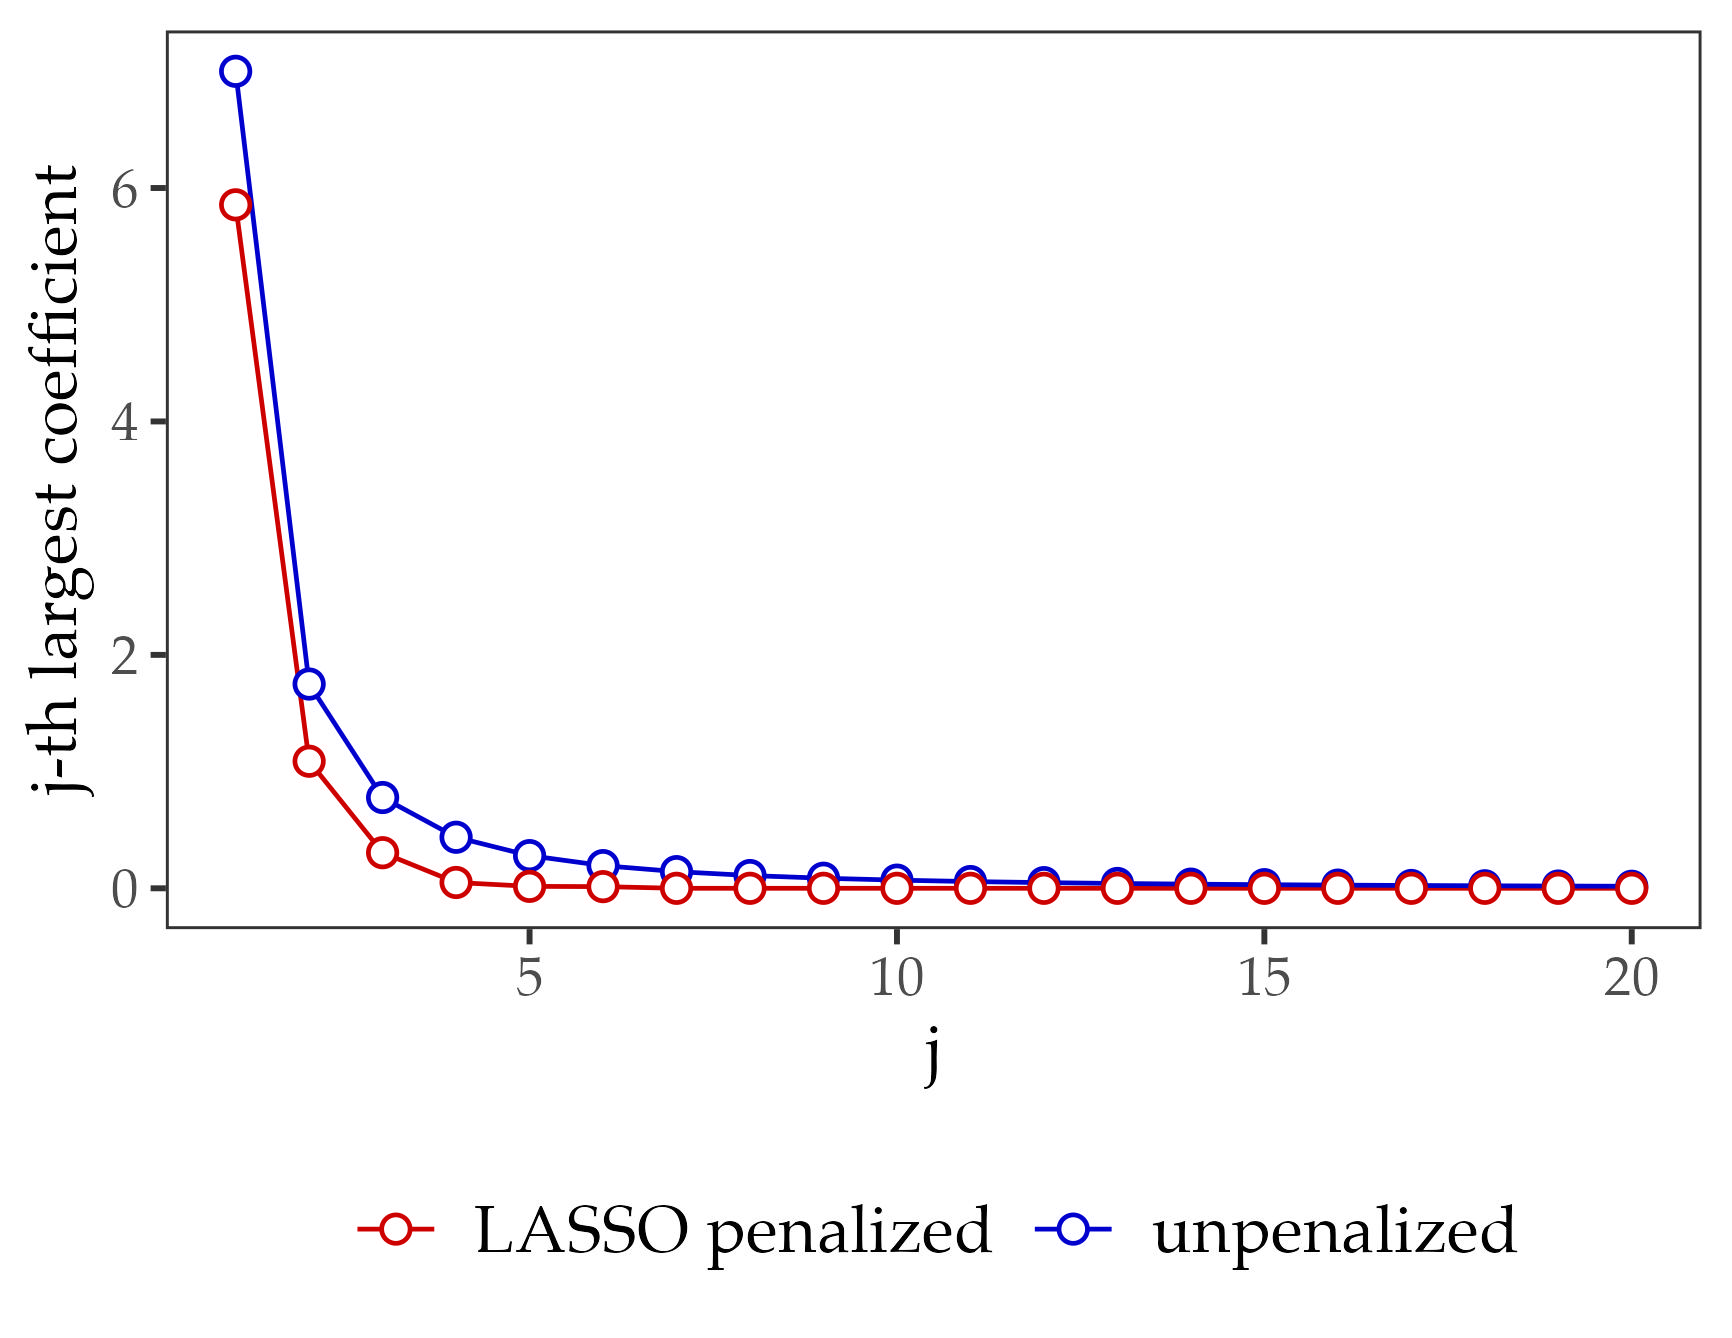
\includegraphics[width=0.6\linewidth]{Machine Learning Basics/Figures/Figure 3.2.jpg}
    \label{fig:figure3.2}
\end{figure}
    
\end{frame}

\begin{frame}{LASSO Regression Caveats}

\begin{itemize}
    \item The estimates shrink towards zero relative to the unpenalized regression; this is referred as \textit{shrinkage bias} or \textit{regularization bias}
    \item LASSO estimates are therefore (slightly) biased, by design, under \textit{approximate sparsity} \pause
    \item LASSO will not generally select the ``right'' set of variables
    \item Instead, LASSO will tend to exclude variables with small, but non-zero population coefficients
    \item LASSO will tend to fail to select the right variables in settings where the $X_i$ variables are corrected
\end{itemize}
\end{frame}

\begin{frame}{LASSO Regression Caveats}

\begin{itemize}
    \item For example, consider a scenario where variable $X_1$ has coefficient $\beta_1=0$ but is highly correlated to variables $X_2,...,X_k$ that have non-zero coefficients
    \item It is plausible that the marginal predictive benefits of including $X_1$ in the model is very high when $X_2,...,X_k$ are not in the model, while the marginal predictive benefits of any one of $X_2,...,X_k$ is relatively low
    \item In this case, $X_1$ may enter the LASSO solution with a non-zero coefficient, while all of $X_2,...,X_k$ are excluded
    \item This inability to select \textit{exactly} the right regressors is not special to LASSO but shared by all variable selection procedures
\end{itemize}
\end{frame}

\begin{frame}{Post-LASSO Regression}

\begin{itemize}
    \item One way to adjust for the \textit{shrinkage bias} of LASSO is to refit the OLS model using the regressors whose LASSO coefficient estimates are non-zero
    \item This method is called ``least squares post LASSO'', or simply \textit{Post-LASSO}
    \item Correcting for the \textit{shrinkage} towards zero from the non-zero coefficients sometimes delivers improvements in predictive performance 
    \begin{align*}
        \hat \beta_{post} = \argmin_{b\in\mathbb{R}^p} \sum_{i}(Y_i - X_i'b)^2 \text{ such that } b_j=0 \text{ if } \hat{\beta}_j = 0
    \end{align*}
    where $\hat \beta$ is the LASSO coefficient estimator
\end{itemize}
\end{frame}

\begin{frame}{Post-LASSO Regression}

\begin{figure}
    \centering
    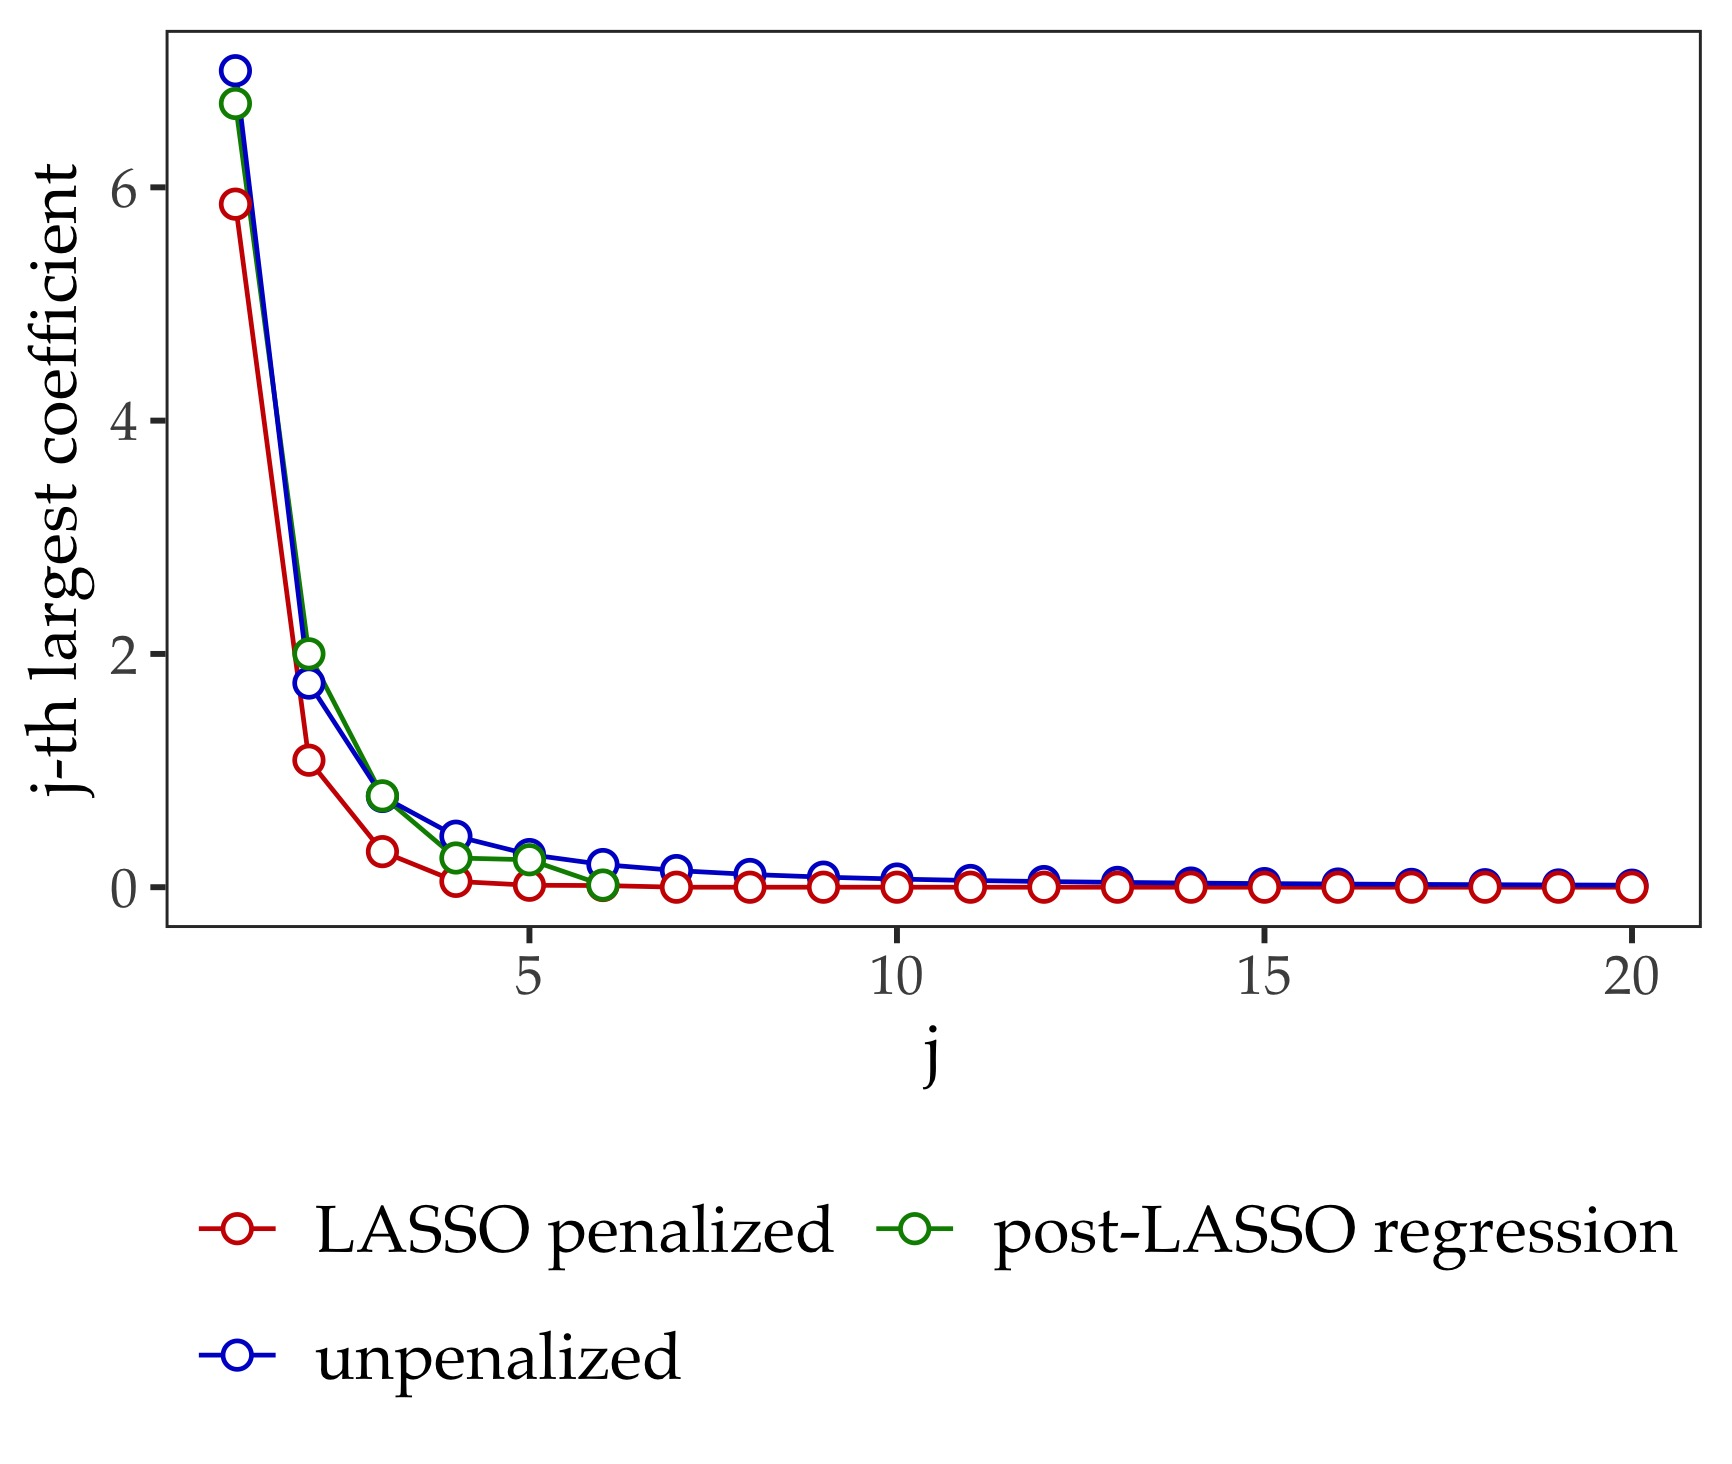
\includegraphics[width=0.6\linewidth]{Machine Learning Basics/Figures/Figure 3.3.jpg}
    \label{fig:figure 3.3}
\end{figure}
\end{frame}

\begin{frame}{Predictive Performance of LASSO and Post-LASSO}

\begin{itemize}
    \item Recall that, \textit{without} feature selection, \textit{out-of-sample} prediction from OLS estimates are poor in high-dimensional regime
    \[
    \sqrt{E_X\!\big[(X_i'\beta - X_i'\hat\beta)^2\big]}
    \lesssim\text{const}_{\alpha}\,\sqrt{E[e_i^2]}\,\sqrt{\tfrac{p}{n}}
    \]
    \item Intuitively, by reducing dimension $p$ to $s$ (\textit{effective dimension}) using LASSO, \textit{out-of-sample} prediction improves
    \[
    \sqrt{E_X\!\big[(X_i'\beta - X_i'\hat\beta)^2\big]}
    \lesssim\text{const}_{\alpha}\,\sqrt{E[e_i^2]}\,\sqrt{\tfrac{s}{n}\log(max\{p,n\})}
    \]
\end{itemize}
\end{frame}

\subsection{Other Penalized Regression Methods beyond LASSO}

\begin{frame}
  \subsectionpage
\end{frame}

\begin{frame}{Other Penalized Regression Methods beyond LASSO}

\begin{itemize}
    \item LASSO performs well in \textit{out-of-sample} prediction when \textit{population}-level DGP follows \textit{approximate sparsity}
    \item Other DGPs exist; for example, a \textit{dense} coefficient vector may have the vast majority or all coefficients non-zero and of \textit{comparable} magnitude
    \item A \textit{sparse and dense} structure has the vast majority of coefficients being non-zero and of similar magnitude along with a small number of relatively large coefficients
\end{itemize}
\end{frame}

\begin{frame}{Other Penalized Regression Methods beyond LASSO}

\begin{figure}
    \centering
    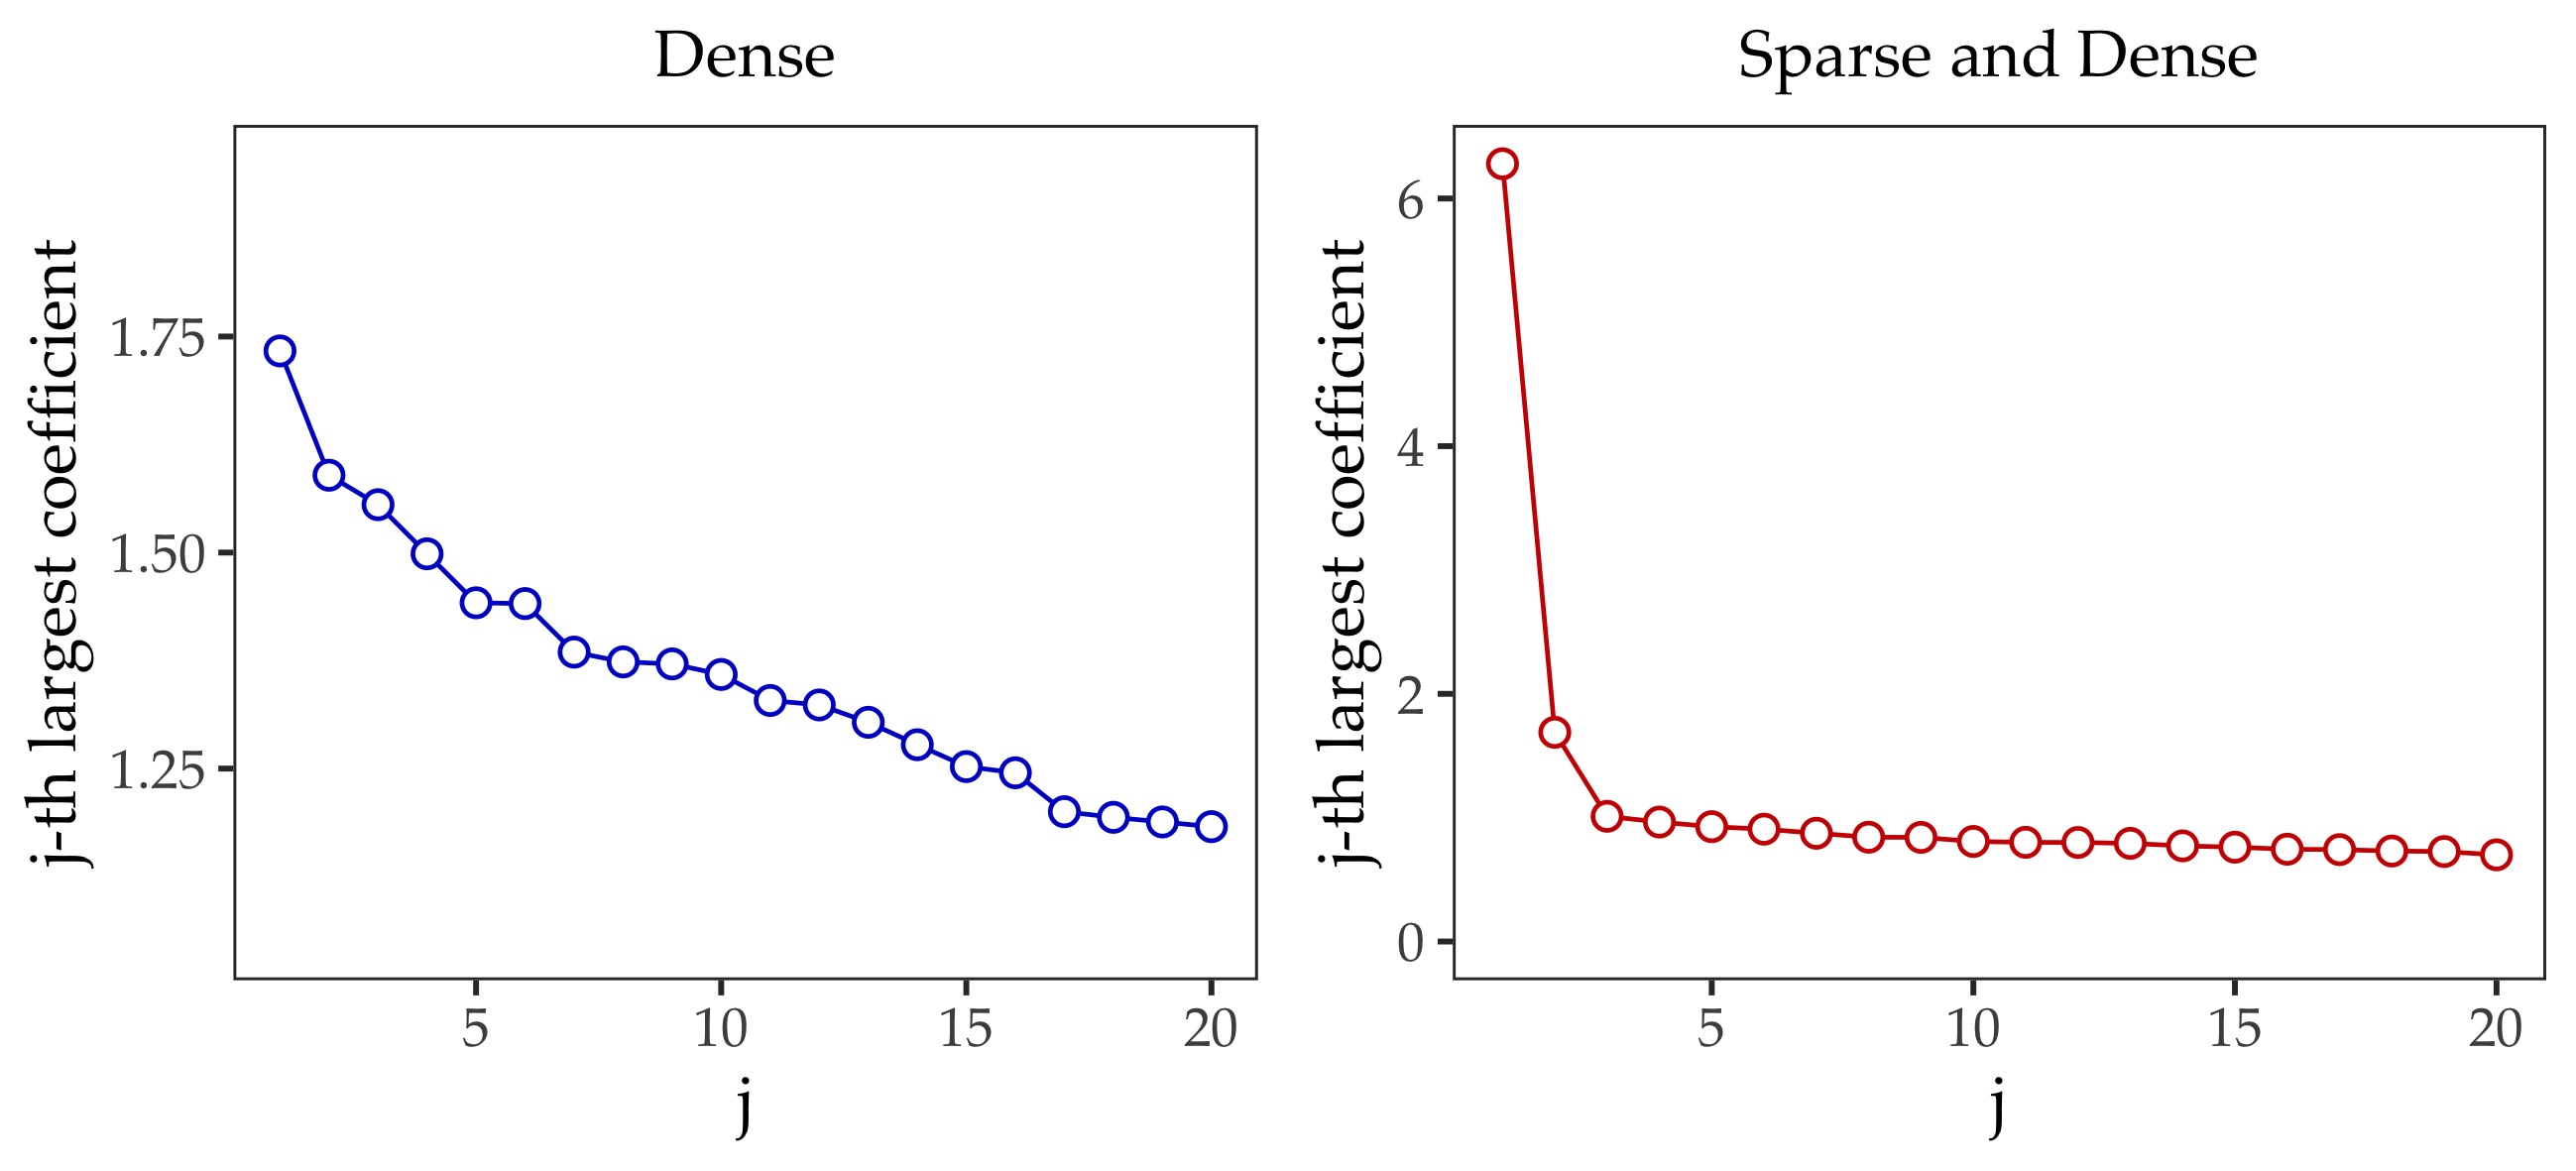
\includegraphics[width=0.9\linewidth]{Machine Learning Basics/Figures/Figure 3.4.jpg}
    \label{fig:figure 3.4}
\end{figure}
\end{frame}

\begin{frame}{Ridge Regression for Dense Coefficients}

\begin{itemize}
    \item While LASSO performs best in an \textit{approximately sparse} setting
    \item Ridge method performs best in the \textit{dense} setting
    \begin{align*}
        \hat \beta = \argmin_{b\in\mathbb{R}^{p}}\sum_i^n(Y_i - X_i'b)^2 + \lambda \cdot \sum_{j=1}^{p}b_j^2
    \end{align*}
    \item The latter penalty term is called $\ell_2$ sphere
    \item In contrast to LASSO, Ridge penalizes the large values of coefficients much more aggressively and small values much less aggressively (to approximate the \textit{dense} DGP)
\end{itemize}
\end{frame}

\begin{frame}{Ridge Regression for Dense Coefficients}

\begin{itemize}
    \item Ridge does not set estimated coefficients to zero and does not do variable selection
    \item In matrix form
    \begin{align*}
        \hat \beta_{Ridge} = (X'X + \lambda I_p)^{-1}X'y
    \end{align*}
    \item Even if $X'X$ is singular (when $p>n$), adding $\lambda I_p$ makes it strictly positive definite and thus invertible
    \item The ridge solution is unique and numerically stable even in high dimension
\end{itemize}
\end{frame}

\begin{frame}{Elastic Net for Sparse \textit{or} Dense Coefficients}

\begin{itemize}
    \item Ridge and LASSO can be combined and perform well in either \textit{sparse} or \textit{dense} settings
    \item One popular hybrid is the Elastic Net with appropriate \textit{tuning} of $\lambda$
    \begin{align*}
        \hat \beta_{Elastic} = \argmin_{b\in\mathbb{R}^{p}}\sum_i^n(Y_i - X_i'b)^2 + \lambda_1 \cdot \sum_{j=1}^{p}b_j^2 + \lambda_2 \cdot \sum_{j=1}^{p}|b_j| 
    \end{align*}
    \item By selecting different values of penalty levels $\lambda_1$ and $\lambda_2$, we have more flexibility with Elastic Net for building a good prediction rule than with just Ridge or LASSO
    \item The Elastic Net performs variable selection unless we completely shut down the LASSO penalty by setting $\lambda_2=0$
\end{itemize}
\end{frame}

\begin{frame}{Lava for Sparse \textit{and} Dense Coefficients}

\begin{itemize}
    \item Ridge and LASSO can also be combined and perform well in \textit{sparse and dense} settings
    \item One such hybrid is the Lava method with appropriate \textit{tuning} of $\lambda$
    \begin{align*}
        \hat \beta_{Lava} = \argmin_{b:b=\delta+\xi\in\mathbb{R}^{p}}\sum_i^n(Y_i - X_i'b)^2 + \lambda_1 \cdot \sum_{j=1}^{p}\delta_j^2 + \lambda_2 \cdot \sum_{j=1}^{p}|\xi_j| 
    \end{align*}
    \item Here components of the parameter vector are split into a ``dense part'' $\delta_j$ and ``sparse part'' $\xi_j$
    \item The minimization program automatically determines the best split into the dense and sparse parts
\end{itemize}
\end{frame}

\begin{frame}{High-Dimensional Linear Model Simulation}

\begin{itemize}
    \item I simulate three high-dimensional ($n=100$, $p=400$) scenarios, where the coefficients in \textit{population} DGP is \textit{dense}, \textit{sparse}, and \textit{dense and sparse}
    \item I \textit{sample} from the \textit{population}, and evaluate the \textit{out-of-sample} prediction by $R^2$
\end{itemize}\vspace{-10pt}
\captionsetup{font=small}
\begin{table}[ht]
\small
\caption{\textit{Out-of-Sample} $R^2$ in Simulation Experiment}
\centering
\begin{tabular}{rccc}
  \hline
 Model & Sparse & Dense & Dense and Sparse \\ 
  \hline
  Lasso (Cross-Validation) & 0.773 & 0.004 & 0.318 \\ 
  Lasso (Plug-in) & 0.775 & -0.028 & 0.329 \\ 
  Post-Lasso (Plug-in) & 0.800 & 0.000 & 0.285 \\ 
  Ridge (Cross-Validation) & 0.097 & 0.170 & 0.116 \\ 
  Elastic Net & 0.741 & 0.005 & 0.319 \\ 
  Lava & 0.770 & 0.159 & 0.399 \\ 
   \hline
\end{tabular}
\end{table}
\end{frame}

\begin{frame}{How to Tune $\lambda$: Cross-Validation}

\begin{itemize}
    \item We want a valid choice of \textit{penalty level} $\lambda$ in these penalized models
    \item Closed-form solution is not always possible
    \item A convenient and theoretically valid choice can be derived from \textit{Cross-Validation} (CV) \pause
    \item Remember our final goal is to find a better \textit{prediction} model after penalizing or selecting regressors under $\lambda$
    \item Intuitively, we can simulate such \textit{prediction} \textit{within} the existing ``training'' sample \textit{without} any test sample
\end{itemize}   
\end{frame}

\begin{frame}{Cross-Validation in Words}

\begin{itemize}
    \item We partition the \textit{sample} data into $K$ blocks called ``folds.'' For example, with $K=5$, we randomly split the data into 5 non-overlapping blocks.
    \item Leave one block out. Fit a prediction rule on all the other blocks. Predict the outcome observations in the left out block, and record the empirical \textit{Mean Squared Prediction Error} (MSE). Repeat this for each block.
    \item Average the empirical MSEs over blocks.
    \item We do these steps for several or many values of the tuning parameters and choose the value of the tuning parameter that minimized the average MSEs.
\end{itemize}   
\end{frame}

\begin{frame}{Cross-Validation Formal Description}

\begin{itemize}
    \item Randomly partition the observation indices $1,...,n$ into $K$ folds $B_1,...,B_K$
    \item For each $k = 1,...,K$, fit a prediction rule denoted by $\hat f ^{-k} (\cdot;\theta)$, where $\theta$ denotes the tuning parameters (\textit{penalty level} $\lambda$ in our case) and $\hat f ^{-k} (\cdot;\theta)$ depends only on observations with indices not in the fold $B_k$
    \item For each $k=1,...,K$, the empirical \textit{out-of-sample} MSE for the block $B_k$ is 
    \[
    MSE_k(\theta) = \frac{1}{m_k} \sum_{i \in B_k} \left( Y_i - \hat f^{-k}(X_i;\theta) \right)^2 \text{ where $m_k$ is the size of the block $B_k$}
    \]
    \item Compute the cross-validated MSE as 
    \[
    CV-MSE(\theta) = \frac{1}{K}\sum_{k=1}^{K} MSE_k(\theta)
    \]
    \item Choose the tuning parameter $\theta$ as a minimizer of $CV-MSE(\theta)$
\end{itemize}   
\end{frame}

\begin{frame}{How to Tune $\lambda$: Plug-in Method for LASSO}

\begin{itemize}
    \item Remember in LASSO, The subgradient condition is satisfied at $\hat\beta_j = 0$ if
    \begin{align*}
        |\hat S_j| \leq \lambda  \text{ where } \hat S_j &= 2\sum_{i=1}^n X_{ji}\Bigl(Y_i - X_{i}'\beta\Bigr) = 2 \sum_{i=1}^n X_{ji}e_i \\
        \mathbb{E}_n[\hat S_j] &= 0, \quad \hat V(\hat S_j) \approx 4n\sigma^2
    \end{align*}
    \item By high-dimensional CLT
    \begin{align*}
        \frac{\hat S_j}{2 \sqrt{n}\sigma} \xrightarrow{d}\mathcal{N}(0,1)
    \end{align*}
    \item We want a $\lambda$ that can check each $j \in \{1,...,p\}$; a theoretically valid $\lambda$ is 
    \[
    \lambda = 2 c \sigma \sqrt{n}z_{1-a/2p}
    \]
    where $1-a$ is a confidence level (with $2p$ adjustments), $c=1.1$ that practically works
\end{itemize}
\end{frame}

\begin{frame}{How to Tune $\lambda$: Plug-in Method for LASSO}

\begin{itemize}
    \item a theoretically valid $\lambda$ is 
    \[
    \lambda = 2 c \sigma \sqrt{n}z_{1-a/2p}
    \]
    \item $\sigma$ can be estimated from iterative method
    \item Let $X_i^{0}$ be a small set of regressors (a trivial choice is just the intercept); fit an unadjusted OLS and find $\hat \beta^0$; we define
    \[
    \hat \sigma^0 := \sqrt{\mathbb{E}_n [Y_i - X_{i}^{0} \hat \beta^0]}
    \]
    \item Compute $\lambda$ using plug-in method based on $\hat \sigma^0$ and LASSO estimator $\hat \beta^1$
    \item Repeat the process for $k$ times until $\hat \sigma^{k+1} - \hat \sigma^{k} \leq v$
    \[
    \hat \sigma^{k} := \sqrt{\mathbb{E}_n [Y_i - X_{i}' \hat \beta^k]}
    \]
\end{itemize}
\end{frame}

\section{Inference in High-Dimensional Linear Regression}

\begin{frame}
  \sectionpage
\end{frame}

\subsection{Inference with Double LASSO}

\begin{frame}{FWL Revisited}

\begin{itemize}
    \item How does the predicted value of $Y_i$ change if $D_i$ increases by a unit, \textit{while holding $W_i$ unchanged}?
\begin{itemize}
    \item What is the difference in predicted wages between men and women with the same characteristics of human capital?
\end{itemize}
    \item In Week 1, we introduced \textit{Frisch-Waugh-Lovell Theorem} (FWL) as a partialling-out method
\begin{align*}
\tilde{Y}_i = \: &\alpha\tilde{D}_i + \tilde{e}_i
\end{align*}
    \item where
    \begin{align*}
        \tilde{D}_i = D_i - \gamma_{DW}' W_i&, \quad
\tilde{Y}_i = Y_i - \gamma_{YW}' W_i \\
\gamma_{DW} = \argmin_{\gamma} E\left[ (D_i - \gamma'W_i)^2 \right]&, \quad
\gamma_{YW} = \argmin_{\gamma} E\left[ (Y_i - \gamma'W_i)^2 \right]
    \end{align*}
\end{itemize}
\end{frame}

\begin{frame}{FWL based on Unpenalized OLS Fails in High Dimension}

\begin{itemize}
    \item Not surprisingly, the unpenalized OLS fails in high dimension ($p/n$ is not small) in the \textit{sample} prediction of $\tilde D_i$ and $\tilde Y_i$
    \item LASSO can be naturally integrated to reduce dimensionality
\end{itemize}
\end{frame}

\begin{frame}{Double LASSO Estimation}

\begin{itemize}
    \item Double LASSO satisfies \textit{Neyman Orthogonality}
    \item Run LASSO regressions of $Y_i$ on $W_i$ and $D_i$ on $W_i$
    \begin{align*}
    \hat \gamma_{YW} &= \argmin_{\gamma \in \mathbb{R}^p} \sum_i^n (Y_i - \gamma'W_i)^2 + \lambda_1 \sum_j^p |\gamma_j| \\
    \hat \gamma_{DW} &= \argmin_{\gamma \in \mathbb{R}^p} \sum_i^n (D_i - \gamma'W_i)^2 + \lambda_2 \sum_j^p |\gamma_j|  \\
    \check{Y}_i &= Y_i - \hat \gamma_{YW}' W_i  \\
    \check{D}_i &= D_i - \hat \gamma_{DW}' W_i
    \end{align*}
\end{itemize}
\end{frame}

\begin{frame}{Double LASSO Estimation}

\begin{itemize}
    \item Double LASSO satisfies \textit{Neyman Orthogonality}
    \item In place of LASSO, we can use Post-LASSO or other LASSO relatives
    \item We run the OLS regression of $\check{Y}_i$ on $\check{D}_i$ to obtain the estimator $\hat \alpha$
    \begin{align*}
        \hat \alpha &= \argmin_{\alpha \in  \mathbb{R}} \mathbb{E}_n [(\check Y_i - \alpha \check D_i)] \\
        &= \frac{\mathbb{E}_n [\check D \check Y]}{\mathbb{E}_n[\check D^2]}
    \end{align*}
    \item Under \textit{Neyman Orthogonality}, the estimation error in $\check Y_i$ and $\check D_i$ has no first-order effect on $\hat{\alpha}$
    \begin{align*}
        \sqrt{n}(\hat \alpha - \alpha) &\xrightarrow{d} \mathcal{N} (0,V) \\
        \text{where } V &= (E[\tilde{D}_i^2])^{-1}E[\tilde{D}_i^2e_i^2](E[\tilde{D}_i^2])^{-1}
    \end{align*}
    \item With $\lambda_1$ and $\lambda_2$ found via plug-in method
\end{itemize}
\end{frame}

\begin{frame}{Double LASSO Estimation}

\begin{itemize}
    \item Good performance of the Double LASSO procedure relies on \textit{approximate sparsity} of the population regression coefficients $\gamma_{YW}$ and $\gamma_{DW}$
    \item With a sufficiently high speed of decrease in the sorted coefficients and on careful choice of the LASSO parameters
    \item Absent these guarantees, we cannot theoretically ensure that the first step estimation of $\check D_i$ and $\check Y_i$ does not have first-order impacts on the final estimator $\hat \alpha$
    \item Practically, LASSO with penalty parameter selected via cross-validation can perform poorly in simulations in moderately sized samples
\end{itemize}
\end{frame}

\begin{frame}{Invalid Single LASSO Estimation (Naive Method)}

\begin{itemize}
    \item Another intuitive but incorrect LASSO estimator only does LASSO once (\textit{Neyman Ortholonality} not satisfied)
    \item One applies LASSO regression of $Y_i$ on $D_i$ and $W_i$ to select relevant covariates $W_Y$, in addition to the covariate of interest, then refits the model using OLS of $Y_i$ on $D_i$ and $W_Y$
\end{itemize}
\end{frame}

\begin{frame}{Double LASSO Demonstration in \textit{R}}

\begin{itemize}
    \item See example of testing the Convergence Hypothesis
\end{itemize}
    
\end{frame}

\begin{frame}{Inference on Many Coefficients}

\begin{itemize}
    \item Consider the model
    \begin{align*}
        Y_i = \sum_{\ell=1}^{p_1} \alpha_{\ell}D_{\ell i} + \sum_{j=1}^{p_2} \beta_j \bar W_j + e_i
    \end{align*}
    \item where we use $D_{\ell}$ for $\ell = 1,...,p_1$ to denote the predictors of interest and $\bar W_{j}$ for $j = 1,...,p_2$ to denote other predictors in the model
\end{itemize}
\end{frame}

\begin{frame}{Inference on Many Coefficients}

\begin{itemize}
    \item There can be at least three motivations for considering many coefficients of interest
    \begin{itemize}
        \item There can be multiple policies whose effect we would like to infer
        \item We can be interested in heterogeneous effects across pre-specified groups
        \item We can be interested in nonlinear effects of policies
    \end{itemize}
\end{itemize}
\end{frame}

\begin{frame}{One-by-One Double LASSO for Many Target Parameters}

\begin{itemize}
    \item Consider the model
    \begin{align*}
        Y_i = \sum_{\ell=1}^{p_1} \alpha_{\ell}D_{\ell i} + \sum_{j=1}^{p_2} \beta_j \bar W_j + e_i
    \end{align*}
    \item For each $\ell = 1,...,p_1$, apply the LASSO procedure for estimation and inference on the coefficient $\alpha_{\ell}$ in the model
    \begin{align*}
        Y_i = \alpha_{\ell} D_{\ell i} + \gamma_{\ell}'W_{\ell} + e_i, \quad W_{\ell} = ((D_{k}')_{k\neq\ell},\bar{W}')'
    \end{align*}
    where $W_{\ell}$ is being partialled out 
\end{itemize}
\end{frame}

\begin{frame}{Other Approaches that Have the Neyman Orthogonality Property}

\begin{itemize}
    \item One way to fix the ``single selection'' approach is to have \textit{double selection}
    \item Find controls $W_{Y}$ that predict $Y_i$ as judged by LASSO
    \item Find controls $W_{D}$ that predict $D_i$ as judged by LASSO
    \item Regress $Y_i$ on $D_i$ and the union of controls $W_{Y} \cup W_{D}$
    \item This procedure is approximately equivalent to the partialling out approach
\end{itemize}
\end{frame}

\begin{frame}{Other Approaches that Have the Neyman Orthogonality Property}

\begin{itemize}
    \item Another procedure that is approximately equivalent to the partialling out approach is \textit{debiased LASSO}
    \item Run a LASSO estimator with suitable choice of $\lambda$ of $Y_i$ on $D_i$ and $W_i$, and save the coefficient estimate $\hat{\beta}$
    \item Run a LASSO estimator with suitable choice of $\lambda$ of $D_i$ on $W_i$, and save the residualized $\check{D_i}$
    \begin{align*}
        \hat{\alpha} = \frac{\mathbb{E}_n[(Y_i - W_i'\hat \beta) \check D_i]}{\mathbb{E}_n[D_i\check D_i]}
    \end{align*}
    \item This is similar to the 2SLS estimator—residualized $\check D_i$ is used to instrument for $D_i$ ($\check D_i \perp W_i$)
\end{itemize}
\end{frame}



\end{document}